\documentclass[a4paper]{article}
\usepackage[utf8]{inputenc}
\usepackage[T1]{fontenc}
\usepackage{url}
\usepackage{tikz}

\title{2-24-1 Optimization and search heuristics}
\author{Baptiste Louf, Yann Ramusat}

\begin{document}
\maketitle

For the purpose of the project we have implemented most of the algorithms seen during the first part of the course.
In addition to the \textit{RLS} and \textit{(1+1)EA} that are already part of the bootstrap project we propose the \textit{($\mu$+$\lambda$)EA}, the \textit{($\mu$,$\lambda$)EA}, the \textit{simulated annealing} and the \textit{1+($\lambda$,$\lambda$)GA}.

We also use an heuristic to identify useless object and delete them. You can find more information for this processing in INSERT REF.

We will discuss about the impact of the preprocessing, the optimal parameters $\lambda$ and $\mu$ for each algorithm and we will compare the differents heuristics over different kind of instances.

\section{Preprocessing}

We begin with a comparison of the effectiveness of the \textit{RLS} with and without the preprocessing. This will give an insight of the utility of this method. We consider the dataset \textbf{fnl4461 n4460 bounded-strongly-corr 01}.

\begin{figure}[!h]
	\begin{center}
		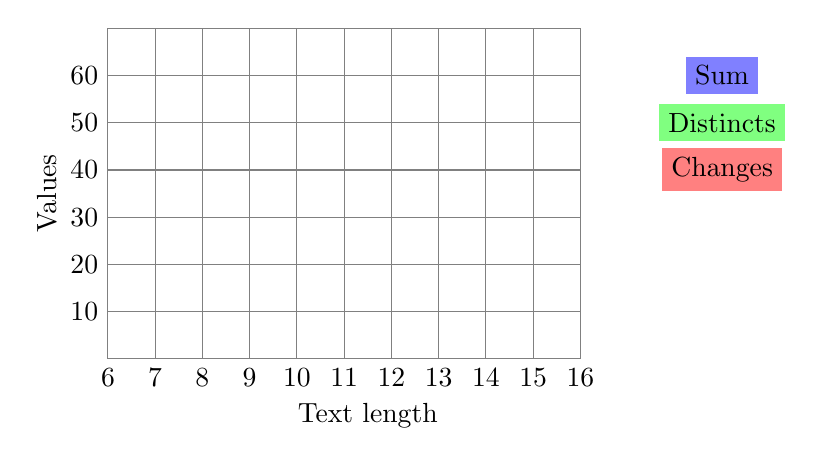
\begin{tikzpicture}[scale = 0.6]
			\draw[step=1,gray,thin]  (0,0) grid (10,7);
			\foreach \x in {6,7,8,9,10,11,12,13,14,15,16}
		 \node[anchor=north] at (\x-6,0) {\x};
			\foreach \y in {10,20,30,40,50,60}
		 \node[anchor=east] at (0,\y/10) {\y};
			\draw (5.5,-1.2) node{Text length};
			\draw (-1.3,3.5) node[rotate=90]{Values};
			
			\draw[thick] plot file {expe_res_m5_s2_black.txt};
			\draw[thick, color=gray] plot file {expe_res_m5_s2_gray.txt};
			\draw[thin, color=blue] plot[mark=*] file {expe_res_m5_s2_blue.txt};
			\draw[thin, color=green] plot[mark=+] file {expe_res_m5_s2_green.txt};
			\draw[thin, color=red] plot[mark=x] file {expe_res_m5_s2_red.txt};
			
			\draw(13,6)node[fill=blue!50] {Sum};
			\draw(13,5)node[fill=green!50] {Distincts};
			\draw(13,4)node[fill=red!50] {Changes};
		\end{tikzpicture}
	\end{center}
	\caption{$S$, $D$ and $C$ function of $n$ for fixed $m=5$ and $\sigma=2$. The black function is $(\sigma-1)m(n-m)$ and the gray one is $m + (\sigma - 1)n$.}
	\label{expe_res_m5_s2}
\end{figure}


\end{document}